\section{Tổng quan trò chơi và kiến trúc}
\label{sec:architecture}

\subsection{Mô hình môi trường tác tử}
\label{subsec:peas}
Để đặt nền móng lý thuyết vững chắc cho việc thiết kế tác tử suy diễn, bài toán điều tra trên lưới trước tiên được hình thức hóa thông qua khung đặc tả môi trường chuẩn mực gồm bốn thành phần: thước đo hiệu năng, môi trường, bộ tác động và bộ cảm biến \cite{russell2020aima}, như được tóm lược trong Bảng \ref{tab:peas_griductive}. Khác biệt căn bản nhất của môi trường này so với các bài toán hoạch định đường đi truyền thống nằm ở tính chất \textbf{quan sát một phần}. Tại mỗi thời điểm trung gian của ván đấu, tác tử hoàn toàn không được phép nhìn thấy thân phận thực sự hay nội dung lời khai của những nhân vật đang úp mặt thẻ; toàn bộ nhận thức của tác tử chỉ giới hạn trong tập hợp các ô đã được mở hợp lệ trước đó.

\begin{table}[H]
\centering
\caption{Đặc tả môi trường tác tử suy diễn trên lưới theo bốn thành phần chuẩn}
\label{tab:peas_griductive}
\small
\begin{tabularx}{\textwidth}{l >{\raggedright\arraybackslash}X}
\toprule
\textbf{Thành phần} & \textbf{Bản chất vận hành trong hệ thống suy diễn} \\
\midrule
\textbf{Thước đo hiệu năng} &
Giải mã chính xác toàn bộ $N^2$ thân phận trên bàn cờ với tỷ lệ suy đoán vô căn cứ bằng không tuyệt đối, đồng thời tối thiểu hóa số lượt gọi bộ giải mệnh đề, số phép lan truyền đơn vị và độ trễ phản hồi ở từng bước lập luận. \\
\midrule
\textbf{Môi trường} &
Bàn cờ vuông rời rạc kích thước $N \times N$ ($N \in \{3, 4, 5\}$) lưu giữ cấu hình thân phận cố định và hệ thống lời khai trung thực mở rộng đơn điệu sau mỗi lần một ô mới được chứng minh thành công. \\
\midrule
\textbf{Bộ tác động} &
Thực hiện phán quyết gán nhãn tội phạm hoặc vô tội lên một tọa độ cụ thể trên lưới, phát gợi ý hợp lệ kế tiếp cho người chơi hoặc điều khiển chu trình giải tự động từng bước đến khi hoàn tất vụ án. \\
\midrule
\textbf{Bộ cảm biến} &
Tiếp nhận bản chụp trạng thái công khai bất biến chứa kích thước lưới, danh sách các thân phận đã được chứng minh và nội dung cấu trúc của các lời khai đã lật mở, tách biệt hoàn toàn khỏi kho đáp án ẩn. \\
\bottomrule
\end{tabularx}
\end{table}

Xét sâu hơn theo các chiều phân loại tính chất môi trường trong lý thuyết tác tử thông minh \cite{russell2020aima}, trò chơi mang tính \textbf{tất định} và \textbf{tuần tự} rất rõ nét. Tính tất định thể hiện ở chỗ mỗi khi một ô được chứng minh hợp lệ, dữ kiện mới lật mở từ ô đó được xác định duy nhất bởi cấu trúc màn chơi mà không hề chịu bất kỳ nhiễu ngẫu nhiên nào; hơn nữa, bản thân quy tắc chọn biến và thứ tự quét lưới của tác tử cũng được thiết kế cố định để bảo đảm tính tái lập hoàn toàn qua mọi lần chạy. Song hành cùng tính tất định là tính tuần tự nhân quả: mỗi kết luận đúng đắn tại bước hiện tại sẽ bổ sung thêm cả khẳng định đơn vị lẫn lời khai mới vào cơ sở tri thức kế tiếp, qua đó thu hẹp không gian mô hình khả dĩ và mở khóa các suy diễn dây chuyền ở những bước về sau. Ngoài ra, môi trường còn mang bản chất \textbf{tĩnh}, \textbf{rời rạc} và \textbf{đơn tác tử}, bởi lẽ bàn cờ không tự biến đổi trong thời gian bộ giải đang suy nghĩ, số lượng biến mệnh đề gốc luôn hữu hạn bằng $N^2$, và không tồn tại đối thủ cạnh tranh làm thay đổi luật chơi.

\subsection{Kiến trúc phân tầng cách ly}
\label{subsec:layered_arch}
Từ yêu cầu bảo toàn tính trung thực của quá trình suy diễn trong môi trường quan sát một phần, nhóm thiết kế kiến trúc phần mềm chia làm năm phân tầng độc lập với chiều phụ thuộc một chiều nghiêm ngặt, được minh họa tổng quan tại Hình \ref{fig:system_architecture}. Triết lý cốt lõi xuyên suốt kiến trúc này là thiết lập một bức tường ngăn cách vật lý giữa phân hệ quản trị trò chơi (nơi lưu giữ đáp án bí mật và các lời khai chưa mở) với phân hệ tác tử suy diễn (nơi thực hiện mã hóa logic và chứng minh mệnh đề). Nhờ cơ chế cô lập này, tác tử giải đố bị tước bỏ hoàn toàn khả năng đọc lén đáp án gốc ngay từ cấp độ cấu trúc dữ liệu, buộc mọi bước tiến trên bàn cờ phải đi qua con đường chứng minh toán học chân chính.

\begin{figure}[H]
\centering
\resizebox{\textwidth}{!}{%
\begin{tikzpicture}[
    node distance=0.8cm and 1.0cm,
    box/.style={rectangle, rounded corners=4pt, draw=black!75, line width=0.7pt, align=center, font=\footnotesize, minimum height=1.05cm, inner sep=6pt},
    privbox/.style={box, fill=red!8, draw=red!65!black},
    pubbox/.style={box, fill=blue!7, draw=blue!65!black},
    logicbox/.style={box, fill=green!8, draw=green!55!black},
    uibox/.style={box, fill=orange!10, draw=orange!70!black},
    arrow/.style={-{Stealth[length=2.4mm,width=1.8mm]}, line width=0.75pt, draw=black!75}
]
    \node[uibox, minimum width=13.2cm] (ui) {
        \textbf{Tầng Giao diện Trực quan Ba chiều (\textit{Midnight Archive})}\\
        \scriptsize Mô phỏng mặt bàn điều tra 3D, chiếu sáng vùng manh mối, đóng dấu trực tiếp lên thẻ và hiển thị thông số giải
    };

    \node[pubbox, below=0.65cm of ui, minimum width=13.2cm] (api) {
        \textbf{Tầng Điều phối Dịch vụ và Kiểm soát Phiên}\\
        \scriptsize Quản lý định danh phiên làm việc, đồng bộ chỉ số phiên bản trạng thái, thẩm định phán quyết và điều phối gợi ý
    };

    \node[privbox, below left=0.85cm and -5.8cm of api, minimum width=5.6cm, minimum height=2.4cm] (engine) {
        \textbf{Tầng Quản trị Trạng thái Ẩn}\\[2pt]
        \scriptsize Cơ sở dữ liệu 14 màn chơi chuẩn\\
        \scriptsize Bộ kiểm định tính trung thực lời khai\\
        \scriptsize \textbf{Lưu giữ độc quyền đáp án gốc}
    };

    \node[logicbox, below right=0.85cm and -5.8cm of api, minimum width=6.6cm, minimum height=2.4cm] (agent) {
        \textbf{Tầng Tác tử Suy diễn Logic}\\[2pt]
        \scriptsize Chỉ tiếp nhận bản chụp trạng thái công khai\\
        \scriptsize Chứng minh phản chứng kết hợp bộ nhớ đệm chứng nhân\\
        \scriptsize Chu trình giải không đoán mò và kiểm định nghiệm duy nhất
    };

    \node[logicbox, below left=0.8cm and -2.85cm of agent, minimum width=2.85cm] (cnf) {
        \textbf{Bộ Mã hóa CNF}\\
        \scriptsize Ràng buộc cơ bản,\\
        \scriptsize đếm lực lượng \& chẵn lẻ
    };

    \node[logicbox, below right=0.8cm and -2.85cm of agent, minimum width=2.85cm] (dpll) {
        \textbf{Bộ Giải DPLL}\\
        \scriptsize Lan truyền đơn vị,\\
        \scriptsize rẽ nhánh \& quay lui
    };

    \node[box, fill=gray!12, below=6.1cm of api, minimum width=13.2cm, minimum height=0.95cm] (domain) {
        \textbf{Tầng Mô hình Tri thức Nền tảng}: Hệ tọa độ lưới, đại số vùng hình học, biểu thức manh mối và trạng thái công khai
    };

    \draw[arrow, <->] (ui.south) -- node[right, font=\scriptsize] {Thông điệp trạng thái \& phán quyết} (api.north);
    \draw[arrow, <->] ([xshift=-3.5cm]api.south) -- node[left, font=\scriptsize] {Mở thẻ đã chứng minh} (engine.north);
    \draw[arrow, <->] ([xshift=3.2cm]api.south) -- node[right, font=\scriptsize] {Yêu cầu thẩm định logic} (agent.north);
    \draw[arrow, dashed, draw=blue!70!black] (engine.east) -- node[above, font=\scriptsize\bfseries, text=blue!70!black] {Chỉ trích xuất} node[below, font=\scriptsize, text=blue!70!black] {trạng thái công khai} (agent.west);
    \draw[arrow, <->] ([xshift=-1.6cm]agent.south) -- (cnf.north);
    \draw[arrow, <->] ([xshift=1.6cm]agent.south) -- (dpll.north);
    \draw[arrow, ->] (cnf.east) -- node[above, font=\tiny] {CNF} (dpll.west);
    \draw[arrow, ->, draw=gray!70] (engine.south) -- (engine.south |- domain.north);
    \draw[arrow, ->, draw=gray!70] (cnf.south) -- (cnf.south |- domain.north);
    \draw[arrow, ->, draw=gray!70] (dpll.south) -- (dpll.south |- domain.north);
\end{tikzpicture}%
}
\caption{Kiến trúc phần mềm năm tầng và ranh giới cách ly tuyệt đối giữa kho đáp án ẩn với tác tử suy diễn}
\label{fig:system_architecture}
\end{figure}

Sự phối hợp giữa tầng điều phối dịch vụ, tầng quản trị trạng thái ẩn và tầng tác tử suy diễn được bảo chứng bằng hai nguyên tắc kiểm soát chặt chẽ. Trước hết, mỗi ô trên bản chụp công khai luôn tuân thủ bất biến đồng bộ ẩn--hiện: một ô hoặc chưa được mở (ẩn đồng thời cả thân phận lẫn lời khai), hoặc đã được chứng minh (hiển thị đầy đủ cả thân phận lẫn lời khai), tuyệt đối không tồn tại trạng thái rò rỉ nửa vời. Bên cạnh đó, hệ thống áp dụng cơ chế kiểm soát tương tranh lạc quan dựa trên chỉ số phiên bản tăng dần sau mỗi lần lật thẻ. Mỗi khi người chơi hoặc giao diện tự động gửi một phán quyết mới kèm theo chỉ số phiên bản hiện hành, tầng điều phối dịch vụ bắt buộc chuyển phán quyết đó sang tác tử suy diễn để kiểm chứng tính hệ quả trên tập manh mối công khai trước. Chỉ khi tác tử xác nhận phán quyết là hệ quả tất yếu duy nhất và chỉ số phiên bản trùng khớp với trạng thái mới nhất, bộ quản trị trò chơi mới chấp thuận mở thẻ và nâng chỉ số phiên bản lên bước kế tiếp; ngược lại, mọi thao tác đoán mò hoặc gửi trùng từ phiên bản cũ đều bị chặn đứng ngay tại cửa ngõ kiểm định.

\subsection{Không gian điều tra ba chiều}
\label{subsec:gui_3d}
Song song với tính chặt chẽ của kiến trúc suy diễn phía máy chủ, nhóm đặc biệt chú trọng xây dựng tầng giao diện người dùng dưới dạng một không gian bàn làm việc thám tử ba chiều toàn màn hình mang phong cách \textit{Midnight Archive} \cite{threejs2025docs}, như được minh họa tại Hình \ref{fig:gui_overview}. Thay vì trình bày lưới ô vuông hai chiều đơn điệu với hàng loạt thanh trạng thái gây nhiễu thị giác, toàn bộ các thẻ hồ sơ nghi phạm được sắp đặt nổi khối trên mặt bàn gỗ óc chó có độ phản xạ vật lý tự nhiên, bao quanh bởi sổ tay ghi chép, kính lúp, bút chì và chiếc đèn bàn khớp nối tỏa ánh sáng vàng ấm áp. Phía xa hậu cảnh là khung cửa sổ đêm mưa được lập trình bằng bộ đổ bóng đồ họa thời gian thực kết hợp các hạt bụi mịn trôi lơ lửng dưới vầng sáng đèn, tạo nên bầu không khí trầm tĩnh và tập trung cao độ cho quá trình phá án.

\begin{figure}[H]
    \centering
    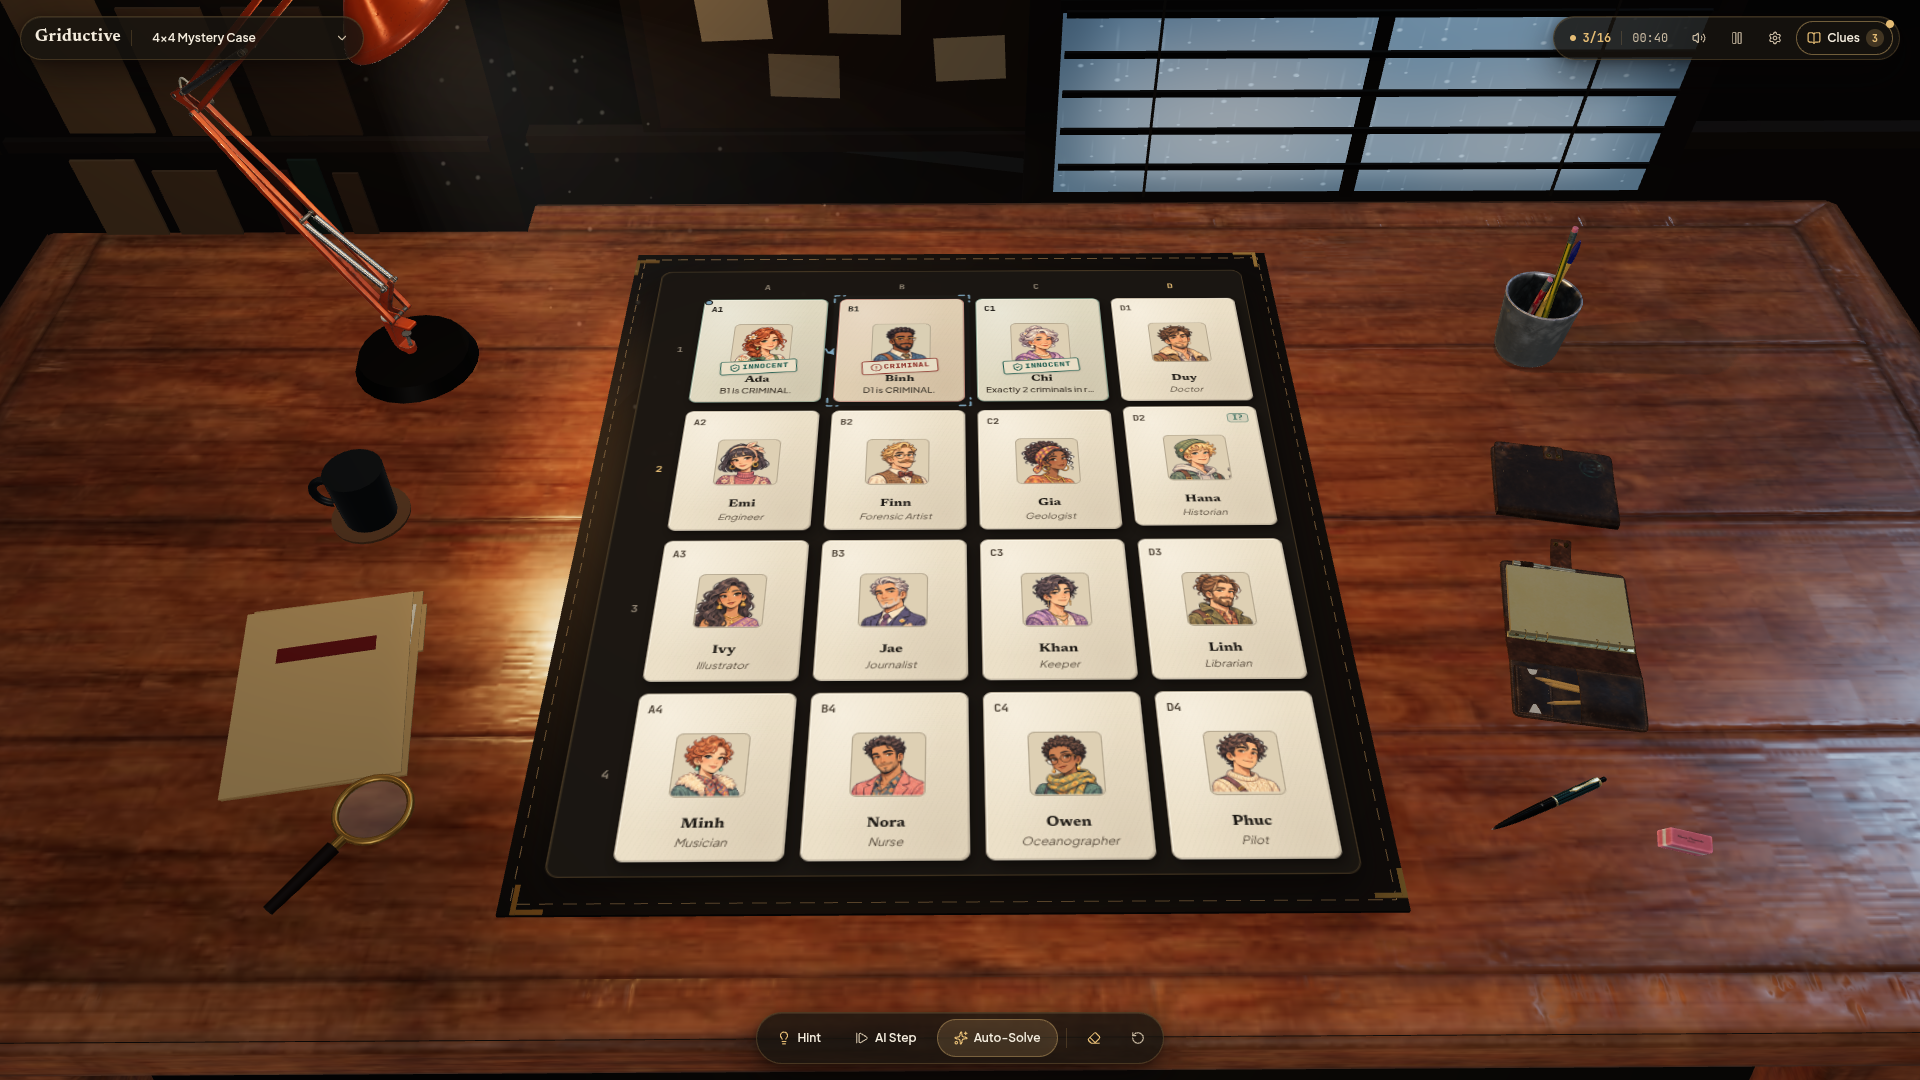
\includegraphics[width=0.92\textwidth]{images/gui_3d_overview.png}
    \caption{Không gian bàn điều tra ba chiều trên màn chơi $4 \times 4$ với các thẻ nghi phạm đã được đóng dấu xác nhận, đạo cụ thám tử và thanh công cụ hỗ trợ suy diễn tối giản}
    \label{fig:gui_overview}
\end{figure}

Để truyền tải trực quan triết lý suy diễn không đoán mò mà không làm gián đoạn mạch tư duy của người chơi bởi các hộp thoại cảnh báo rời rạc, mọi phản hồi logic đều được tích hợp trực tiếp lên bề mặt vật thể trong cảnh ba chiều. Cụ thể, khi người chơi chọn một lời khai trong ngăn kéo manh mối bên phải, hệ thống chiếu sáng trực tiếp đường viền của toàn bộ các thẻ nằm trong vùng không gian chịu sự chi phối của lời khai đó ngay trên mặt bàn. Đáng chú ý hơn, nếu người chơi nôn nóng đưa ra phán quyết cho một nghi phạm khi dữ kiện hiện tại chưa đủ sức chứng minh (chẳng hạn kết luận sớm về ô $\text{B2}$ khi mới chỉ biết một dữ kiện duy nhất tại hàng đầu tiên), một con dấu cao su màu hổ phách mang nhãn chưa thể chứng minh (\textit{``NOT PROVABLE''}) lập tức dập nghiêng trực tiếp xuống mặt thẻ ba chiều kèm hiệu ứng rung nhẹ rồi từ từ tan mực sau gần hai giây (Hình \ref{fig:gui_stamp_and_closed}a). Cuối cùng, khi toàn bộ các mắt xích trên bàn cờ đã được giải mã trọn vẹn, hồ sơ tổng kết vụ án xuất hiện chính giữa màn hình, cung cấp bức tranh định lượng minh bạch về số bước lập luận, tổng số truy vấn SAT, số phép lan truyền đơn vị, số lần quay lui và thời gian thực thi chính xác đến từng phần trăm mili-giây của bộ giải (Hình \ref{fig:gui_stamp_and_closed}b).

\begin{figure}[H]
    \centering
    \begin{subfigure}[t]{0.49\textwidth}
        \centering
        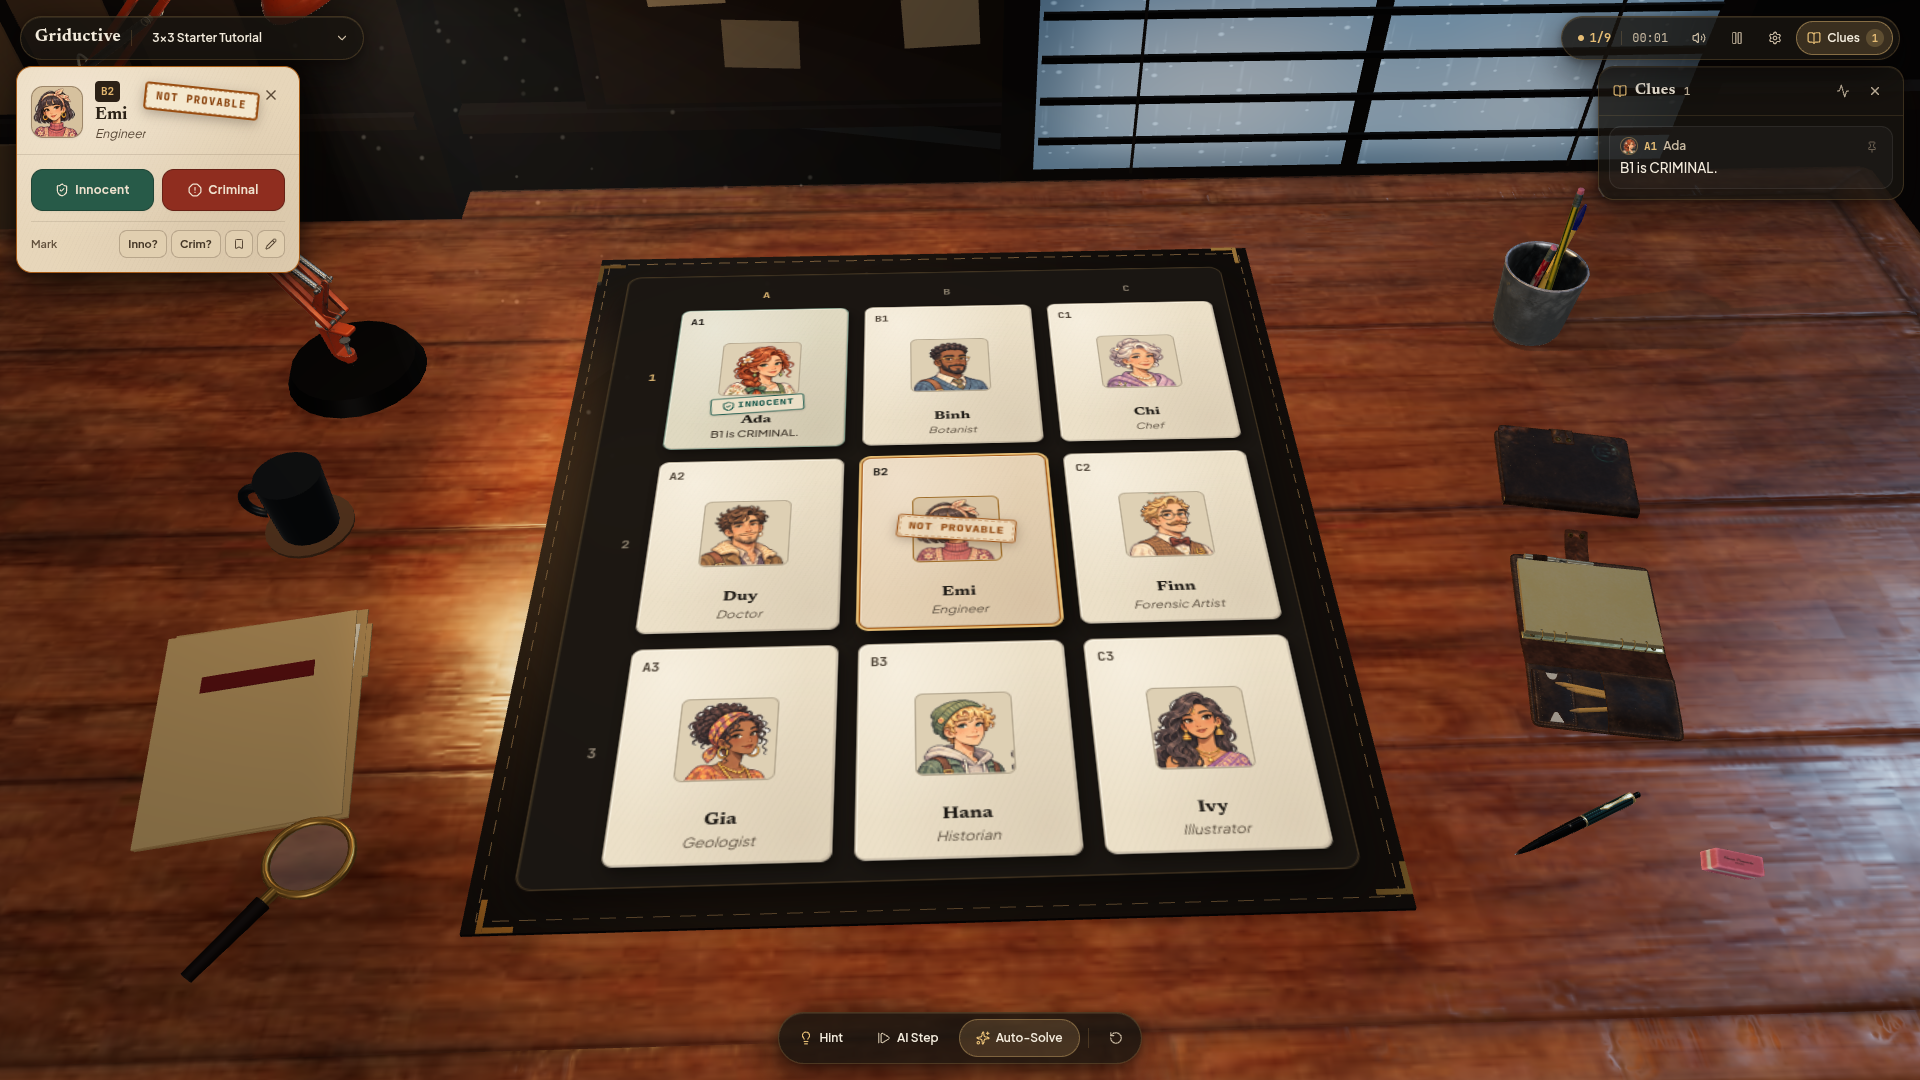
\includegraphics[width=\textwidth]{images/gui_not_provable_stamp.png}
        \caption{Hiệu ứng đóng dấu từ chối trực tiếp lên mặt thẻ $\text{B2}$ khi phán quyết chưa đủ cơ sở chứng minh}
        \label{fig:gui_stamp}
    \end{subfigure}
    \hfill
    \begin{subfigure}[t]{0.49\textwidth}
        \centering
        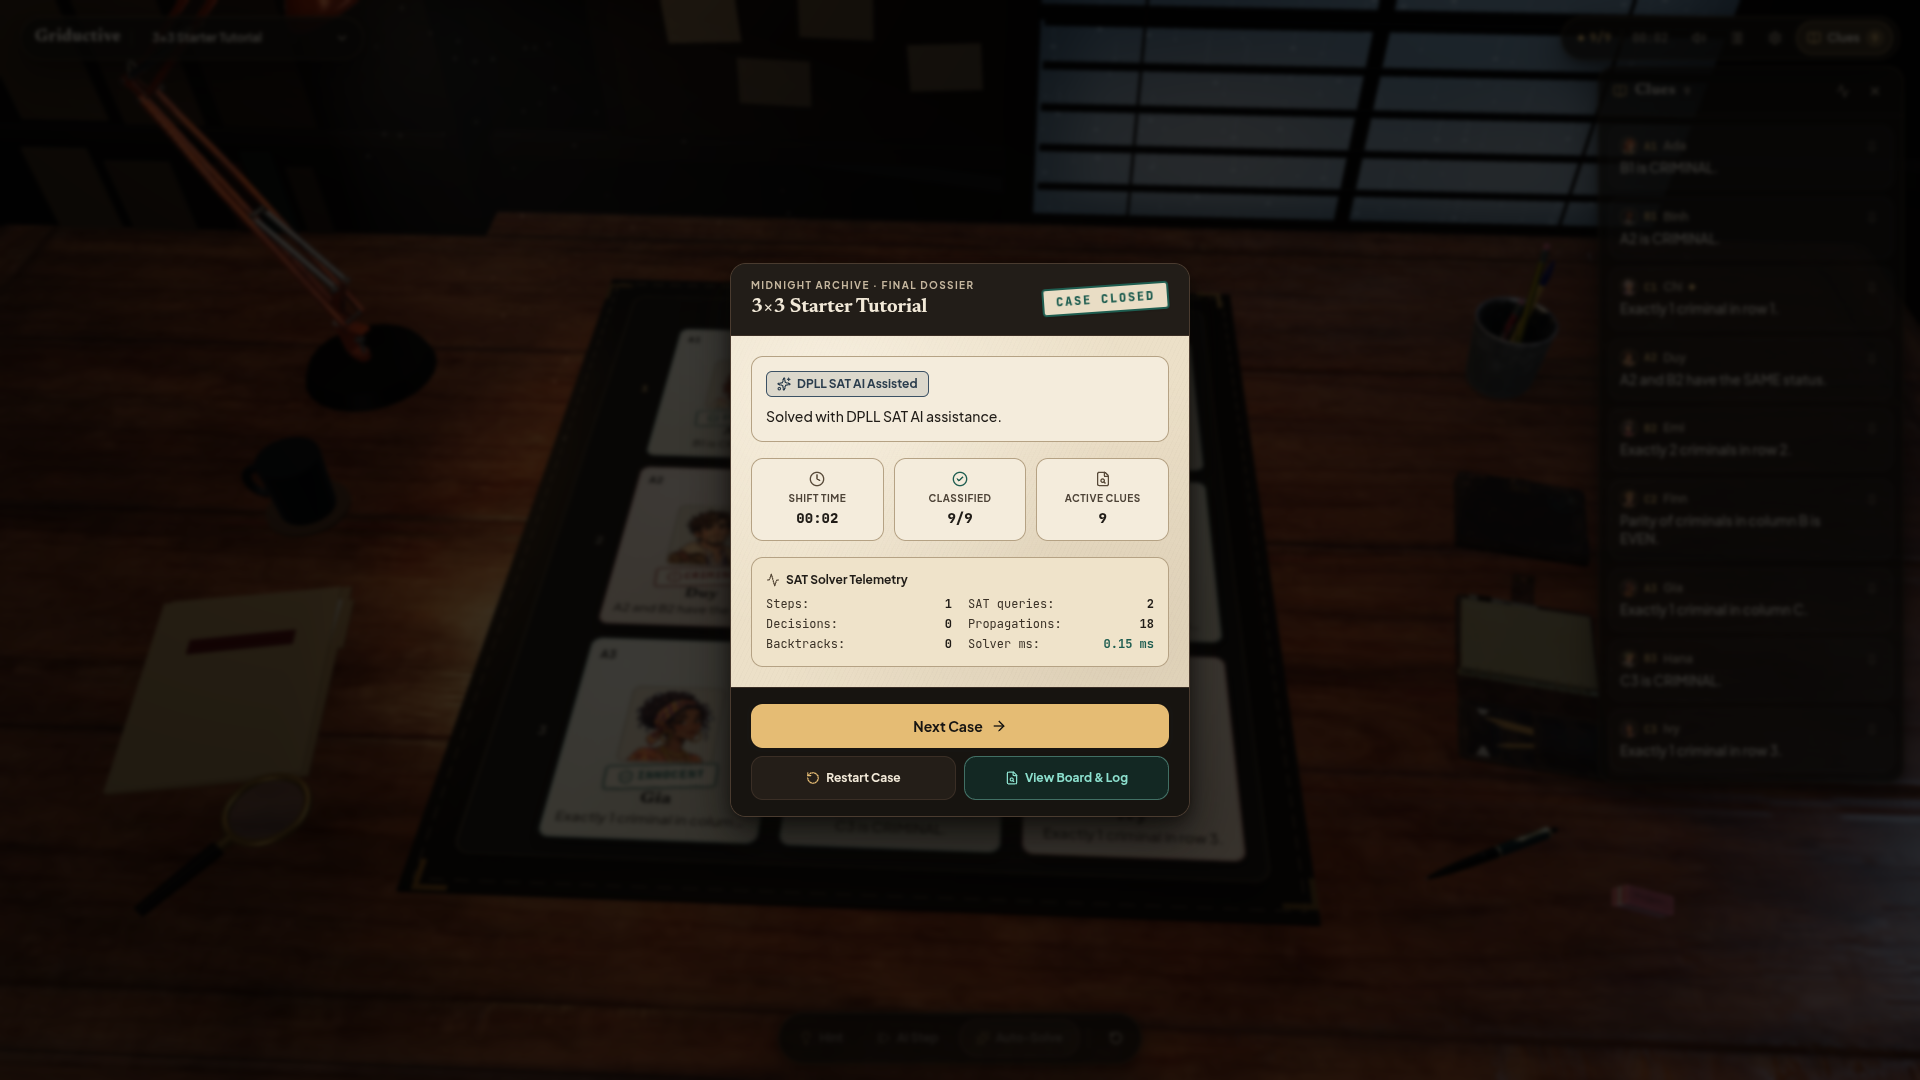
\includegraphics[width=\textwidth]{images/gui_case_closed.png}
        \caption{Hồ sơ khép lại vụ án hiển thị đầy đủ các chỉ số đo đạc vi mô của bộ giải mệnh đề}
        \label{fig:gui_closed}
    \end{subfigure}
    \caption{Phản hồi đóng dấu trực tiếp trên vật thể ba chiều và bảng thống kê thực thi sau khi hoàn tất suy diễn}
    \label{fig:gui_stamp_and_closed}
\end{figure}
